\section{Data Understanding · Explorando los datos}

\begin{takeaway}
Antes de modelar, hay que mirar. Esta fase busca respuesta a tres preguntas:
\textbf{(i)} ¿las ventas son estables o tienen estacionalidad marcada?,
\textbf{(ii)} ¿hay correlaciones entre los canales que puedan confundir al modelo?, y
\textbf{(iii)} ¿los eventos comerciales dejan huella medible?
\end{takeaway}

\subsection{Distribución del target y estacionalidad}

\begin{figure}[htbp]
\centering
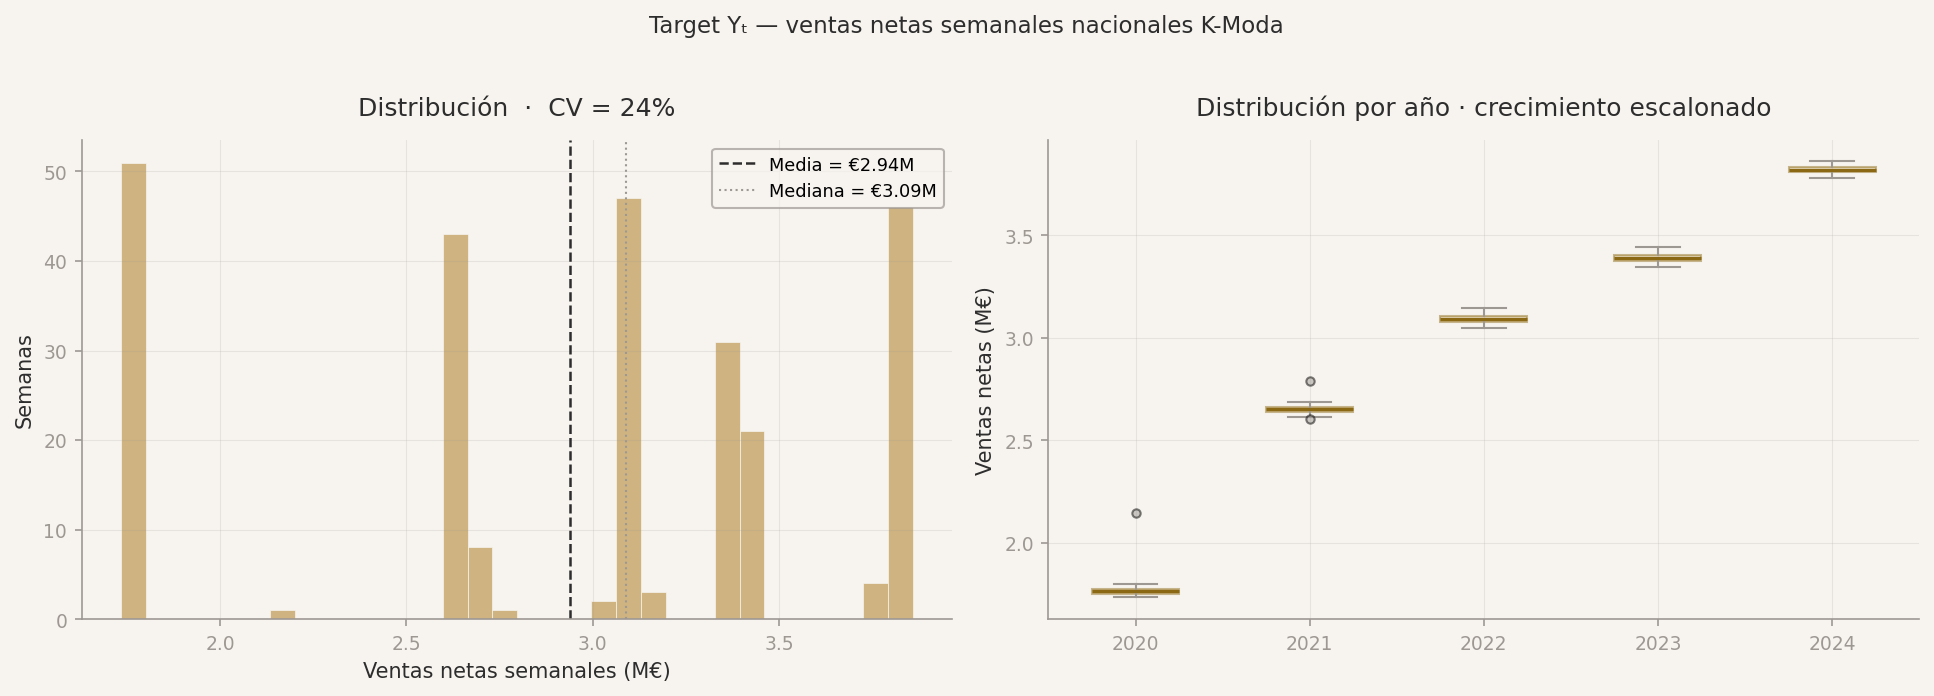
\includegraphics[width=0.95\textwidth]{figures/du_g1_distribucion.png}
\caption{\textbf{Distribución de ventas semanales.} La asimetría a la derecha (cola larga) refleja los picos puntuales de campañas fuertes; el grueso de las semanas se concentra alrededor de la mediana.}
\label{fig:du_dist}
\end{figure}

\begin{figure}[htbp]
\centering
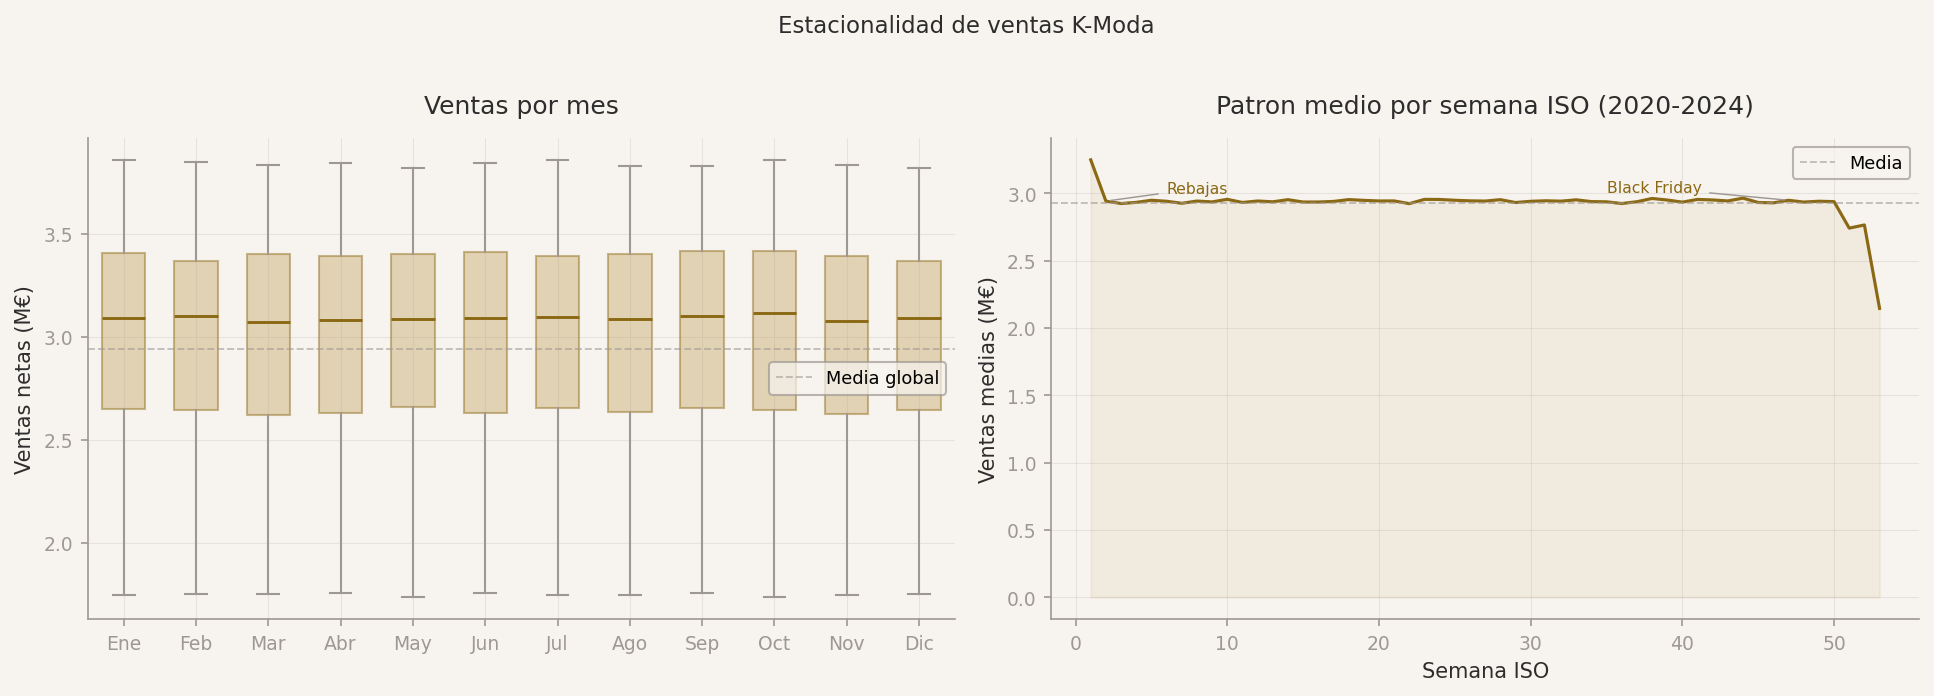
\includegraphics[width=0.95\textwidth]{figures/du_g2_estacionalidad.png}
\caption{\textbf{Estacionalidad anual.} Las ventas repiten un patrón anual reconocible: valles a comienzos de año, crecimiento en primavera, pico en noviembre (\textit{Black Friday}) y otro pico en rebajas de enero.}
\label{fig:du_season}
\end{figure}

\begin{figure}[htbp]
\centering
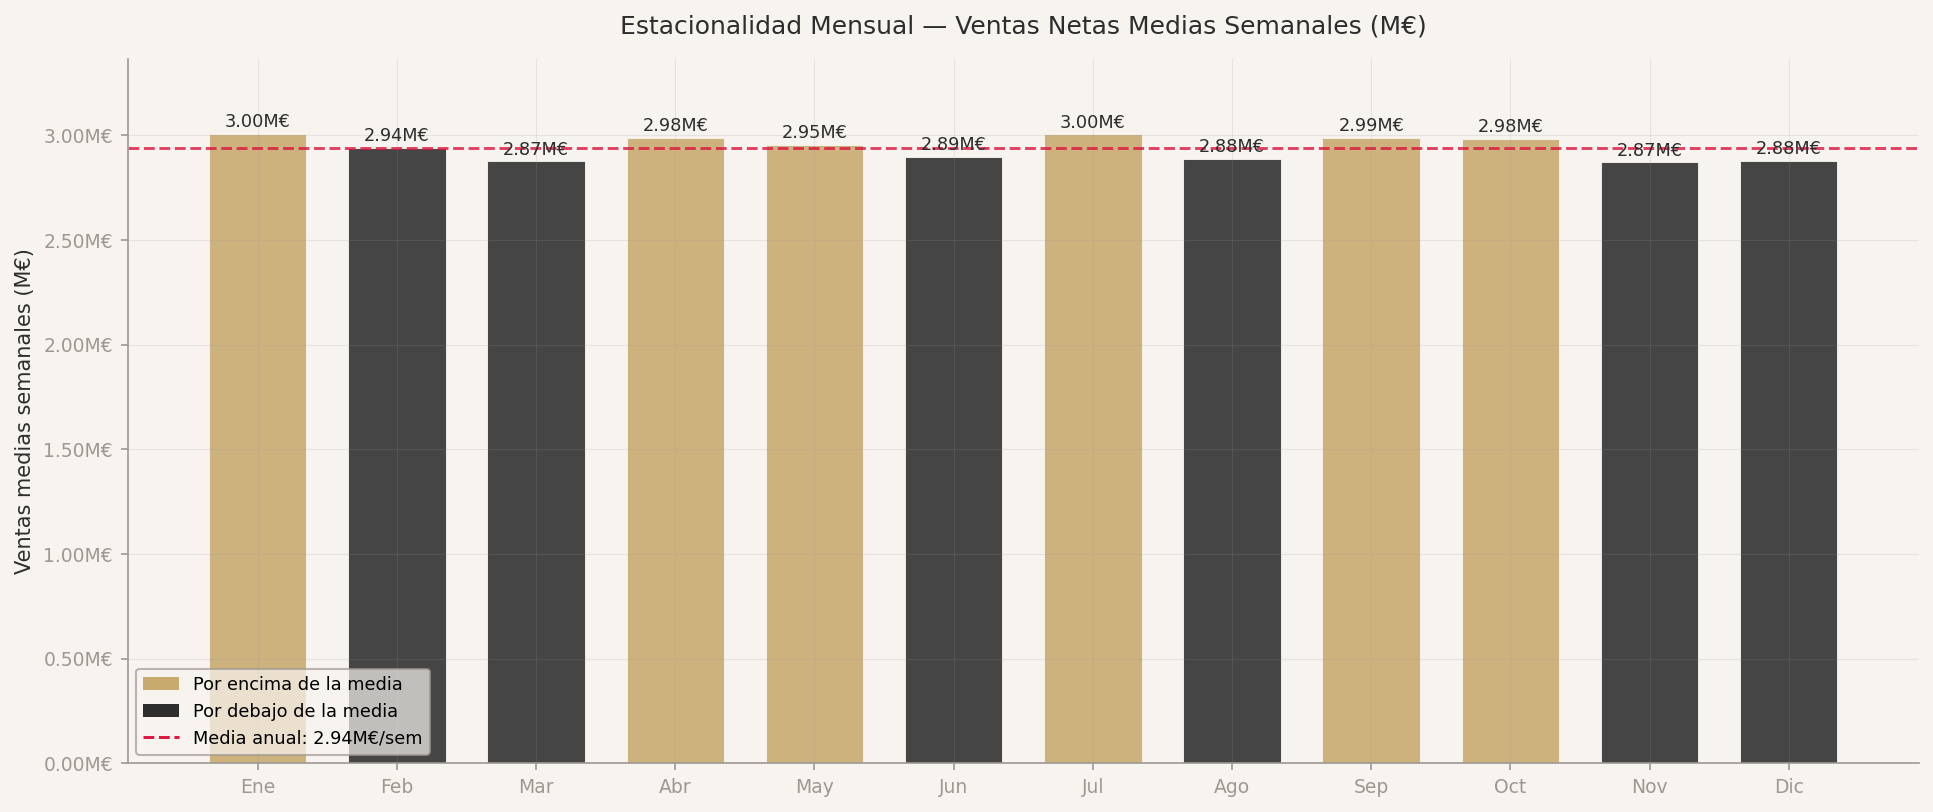
\includegraphics[width=0.95\textwidth]{figures/du_g3b_estacionalidad_mensual.png}
\caption{\textbf{Vista mensual comparada por año.} Permite confirmar que la estacionalidad se mantiene estable en el tiempo — no es un artefacto de un único año.}
\label{fig:du_mensual}
\end{figure}

\begin{figure}[htbp]
\centering
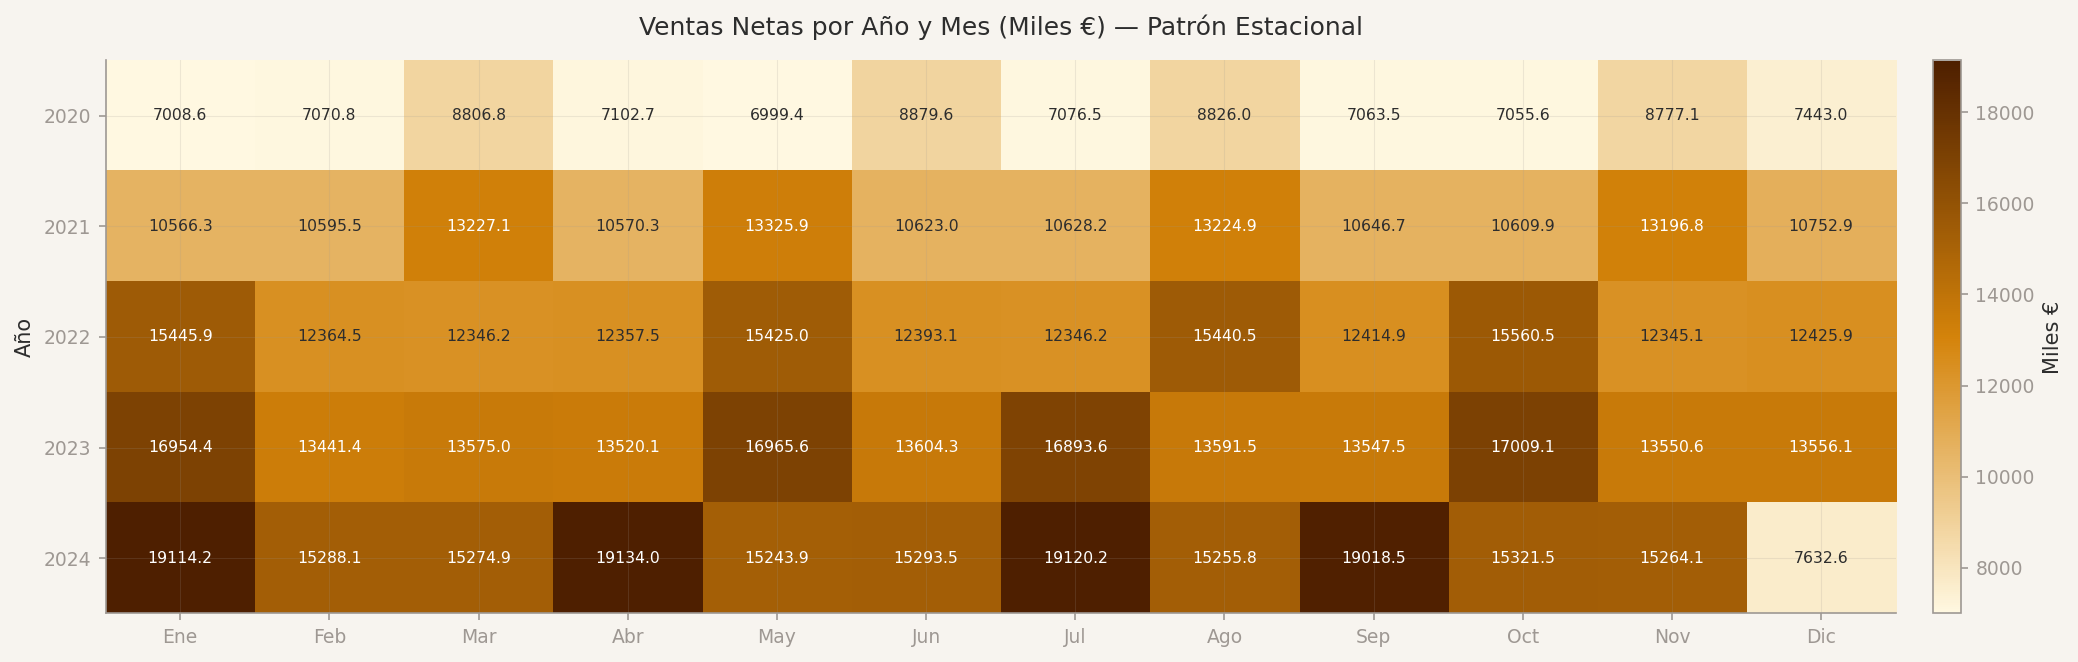
\includegraphics[width=0.95\textwidth]{figures/du_g4b_heatmap_anio_mes.png}
\caption{\textbf{Heatmap año $\times$ mes.} Verde claro = semanas flojas, dorado intenso = picos. La diagonal de crecimiento y la franja vertical de noviembre son las dos señales más claras.}
\label{fig:du_heatmap}
\end{figure}

\subsection{Presupuesto y mix de inversión}

\begin{figure}[htbp]
\centering
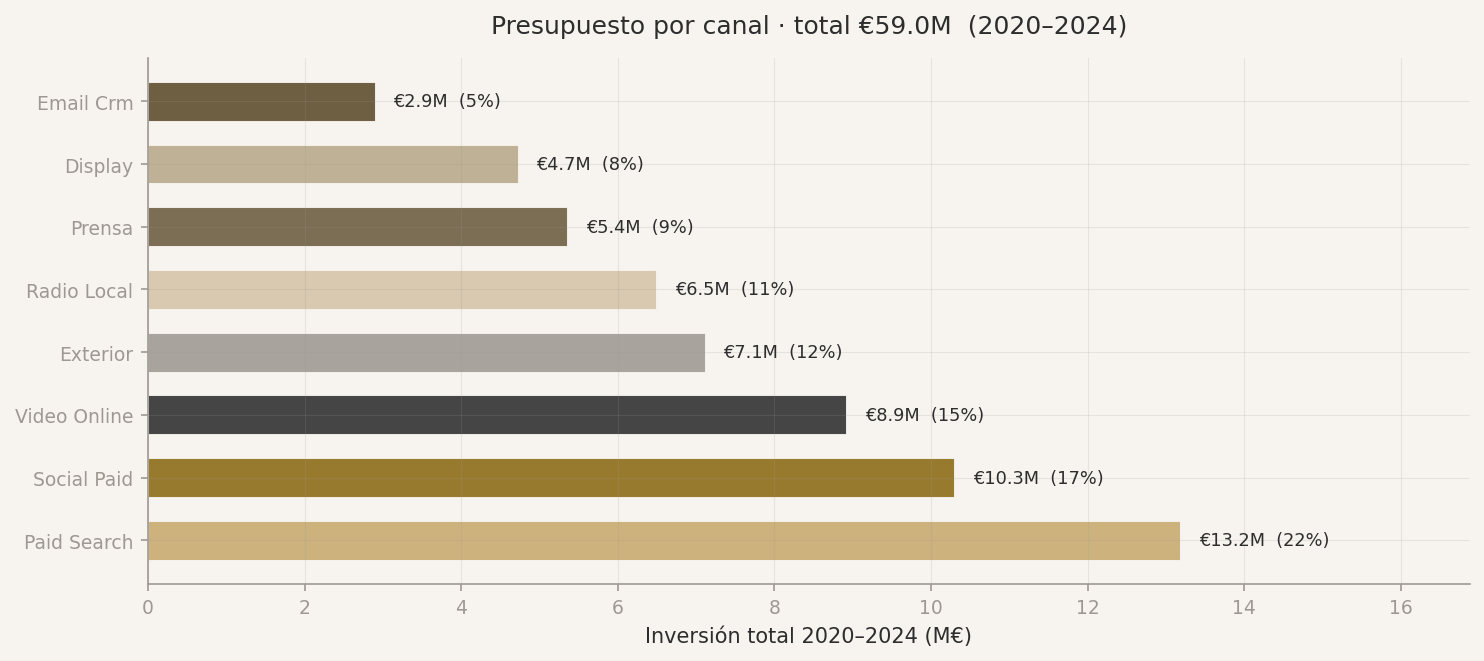
\includegraphics[width=\textwidth]{figures/du_g3_presupuesto.png}
\caption{\textbf{Presupuesto publicitario a lo largo del tiempo.} Cómo ha evolucionado el gasto total y su composición entre canales.}
\label{fig:du_presup}
\end{figure}

\begin{figure}[htbp]
\centering
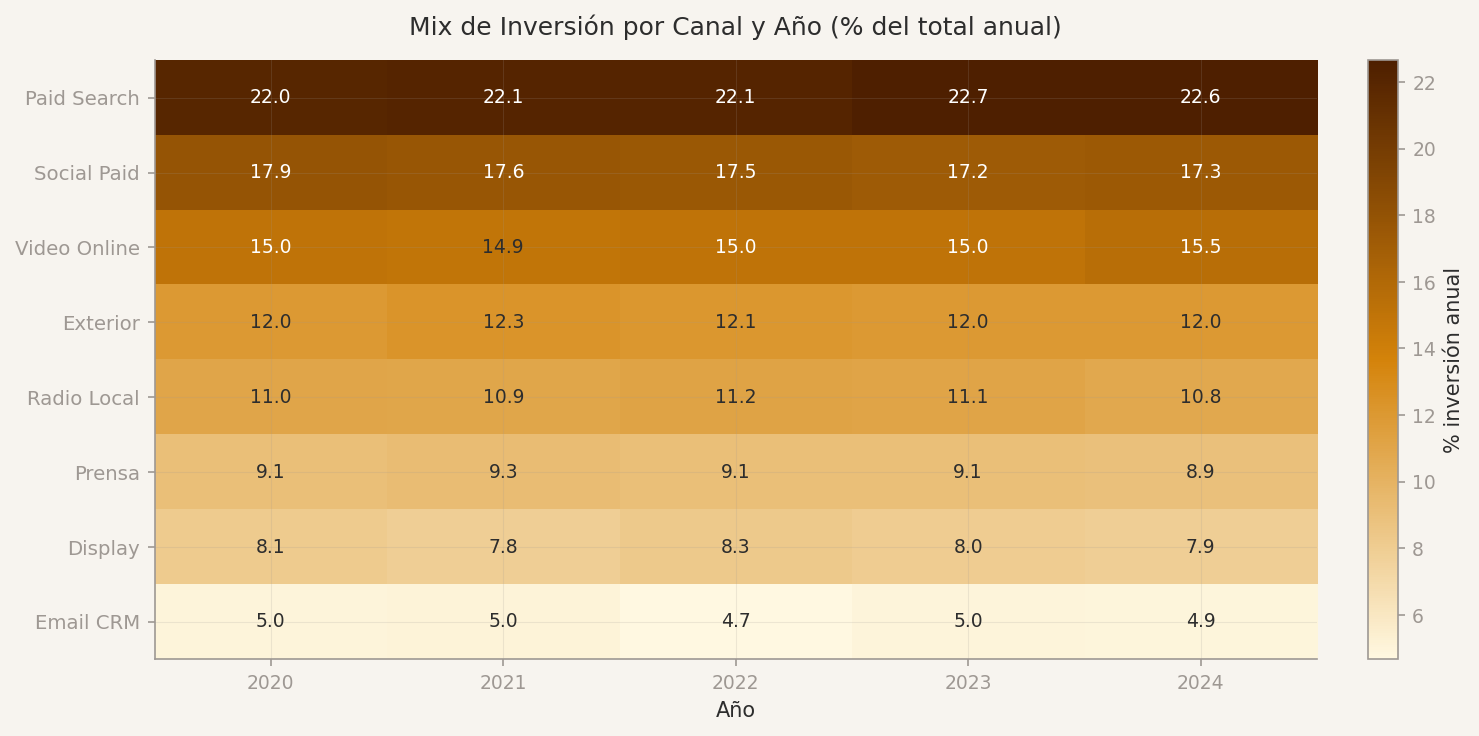
\includegraphics[width=0.95\textwidth]{figures/du_g5b_mix_inversion.png}
\caption{\textbf{Mix porcentual de inversión.} Qué peso relativo tiene cada canal en la cartera total. Este reparto es el \textit{baseline} contra el que se medirán las reasignaciones propuestas.}
\label{fig:du_mix}
\end{figure}

\subsection{Correlaciones y multicolinealidad}

\begin{figure}[htbp]
\centering
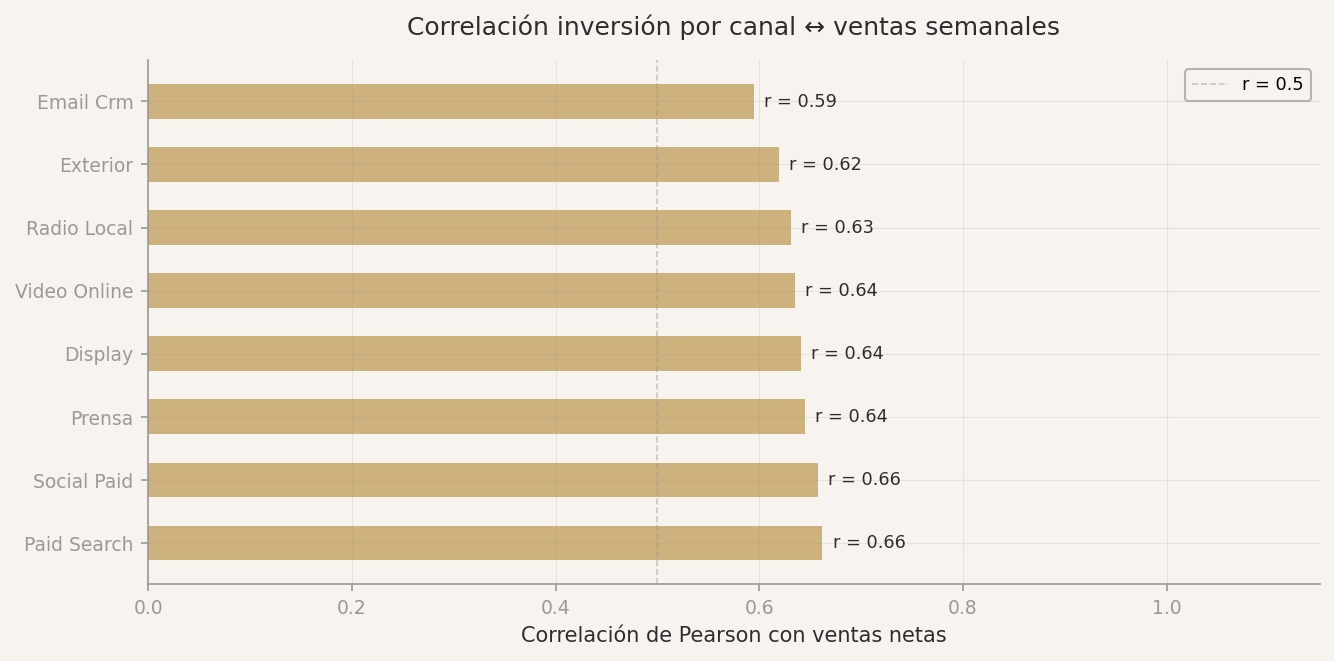
\includegraphics[width=0.9\textwidth]{figures/du_g4_correlacion.png}
\caption{\textbf{Matriz de correlación entre canales de inversión.} Los canales están fuertemente correlacionados entre sí ($\rho$ Spearman $\in [0.83, 0.96]$). Esto adelanta un problema de multicolinealidad que condicionará la decisión de agrupar canales en la fase de \textit{data preparation}.}
\label{fig:du_corr}
\end{figure}

\subsection{Eventos comerciales}

\begin{figure}[htbp]
\centering
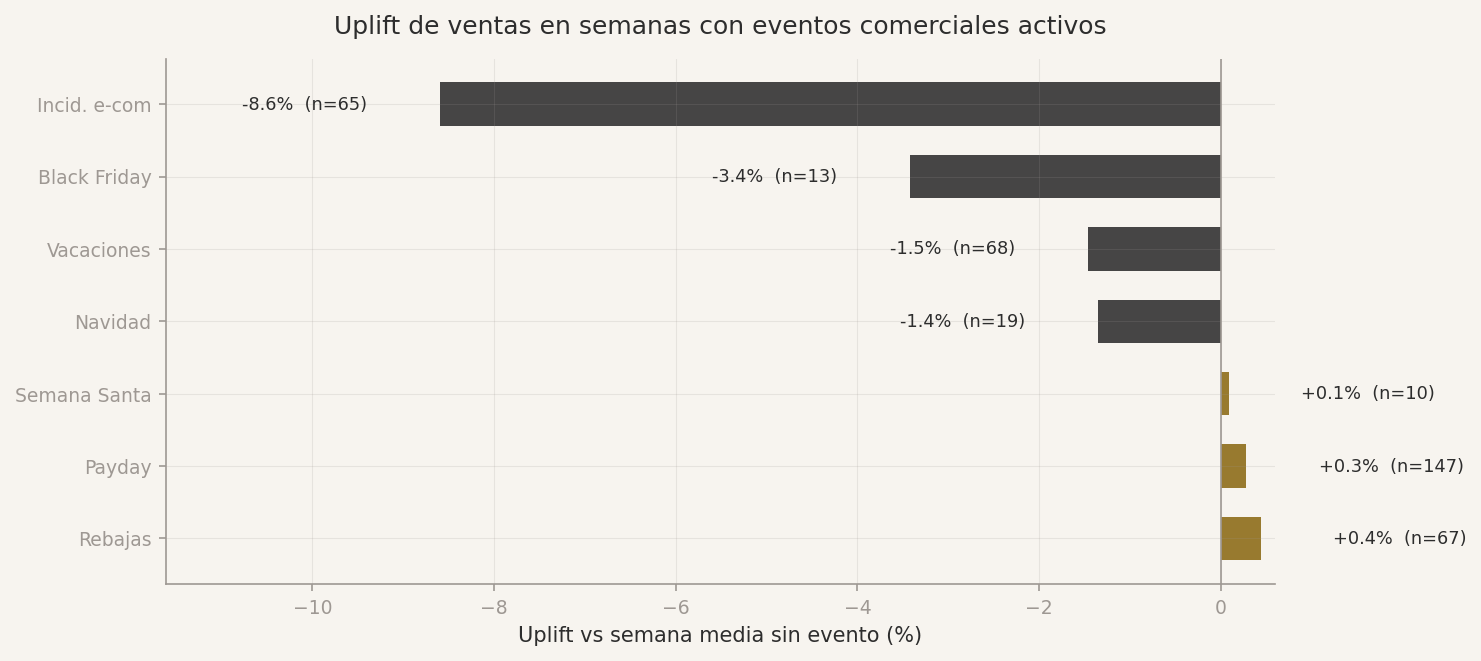
\includegraphics[width=\textwidth]{figures/du_g5_uplift_eventos.png}
\caption{\textbf{Uplift por tipo de evento.} Mediana de ventas en semanas con y sin cada evento. Black Friday y rebajas destacan claramente; Navidad tiene efecto menor porque la preparación se adelanta semanas antes.}
\label{fig:du_uplift}
\end{figure}

\subsection{Autocorrelación del target}

\begin{figure}[htbp]
\centering
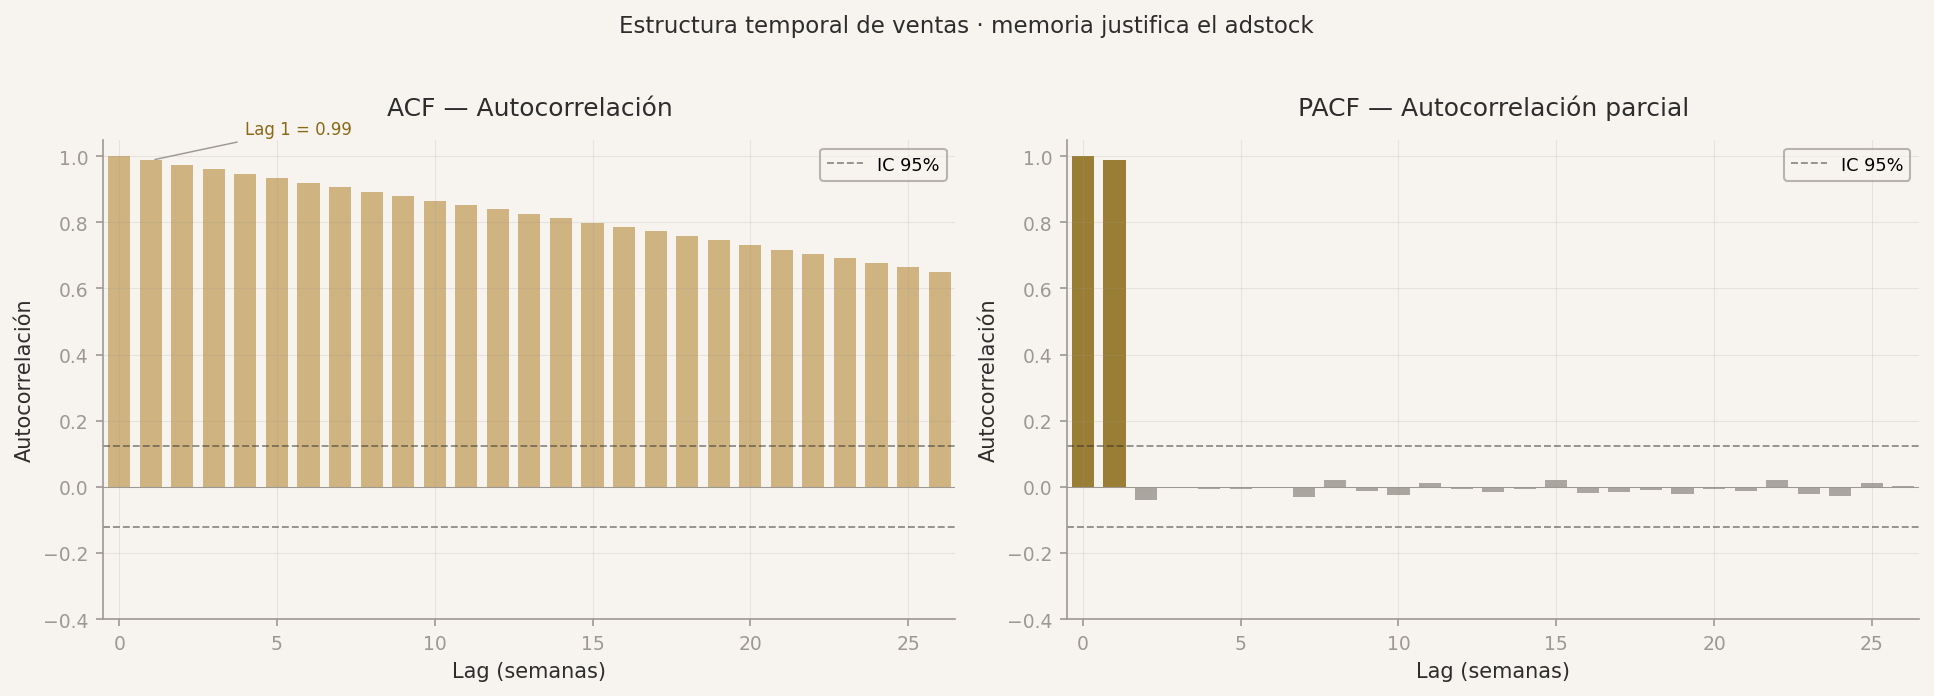
\includegraphics[width=\textwidth]{figures/du_g6_acf_pacf.png}
\caption{\textbf{ACF y PACF del target.} Hay autocorrelación significativa a lag 1 y memoria a largo plazo (componente de tendencia). Ambos elementos se tratan en el preprocesado: la tendencia con las variables de calendario, y la autocorrelación residual con el \textit{block bootstrap} para estimar la incertidumbre de los coeficientes.}
\label{fig:du_acf}
\end{figure}

\subsection{Conclusiones del análisis exploratorio}

\begin{takeaway}
\begin{enumerate}[leftmargin=*, itemsep=2pt]
    \item Las ventas tienen una \textbf{estacionalidad anual reconocible} y un crecimiento estructural año-a-año.
    \item Los canales de inversión están \textbf{muy correlacionados entre sí} — modelar cada canal por separado dará coeficientes inestables.
    \item Los \textbf{eventos comerciales} (Black Friday, rebajas) tienen uplift claro y medible, por lo que deben entrar como controles en el modelo.
    \item El \textbf{tráfico web/tienda} correlaciona con ventas, pero es un mediador: no entra al modelo.
\end{enumerate}
\end{takeaway}
